\documentclass{article}
\usepackage{cmap}
\usepackage[utf8]{inputenc}
\usepackage[english,ukrainian]{babel}
\usepackage{graphicx}
\usepackage{geometry}
\usepackage{listings}
\usepackage{float}
\usepackage{multicol}
\geometry{
	a4paper,
	left=20mm,
	right=20mm,
	top=20mm,
	bottom=20mm
}
\lstset{
	language=c,
	tabsize=4,
	keepspaces,
	showstringspaces=false,
	breaklines,
}
\graphicspath{ {./pictures} }
\setlength{\parindent}{4em}

\newcommand\subject{Алгоритми та структури даних}
\newcommand\lecturer{доцент кафедри ПЗ\\Коротєєва Т.О.}
\newcommand\teacher{асистент кафедри ПЗ\\Франко А.В.}
\newcommand\mygroup{ПЗ-22}
\newcommand\lab{10}
\newcommand\theme{Бінарний пошук в упорядкованому масиві}
\newcommand\purpose{Навчитися застосовувати алгоритм бінарного пошуку при розв’язуванні задач та перевірити його ефективність на різних масивах даних. Експериментально визначити складність алгоритму}

\begin{document}
	\begin{normalsize}
		\begin{titlepage}
			\thispagestyle{empty}
			\begin{center}
				\textbf{МІНІСТЕРСТВО ОСВІТИ І НАУКИ УКРАЇНИ\\
					НАЦІОНАЛЬНИЙ УНІВЕРСИТЕТ "ЛЬВІВСЬКА ПОЛІТЕХНІКА"}
			\end{center}
			\begin{flushright}
				Інститут \textbf{КНІТ}\\
				Кафедра \textbf{ПЗ}
			\end{flushright}
			\vspace{200pt}
			\begin{center}
				\textbf{ЗВІТ}\\
				\vspace{10pt}
				До лабораторної роботи № \lab\\
				\textbf{На тему}: “\textit{\theme}”\\
				\textbf{З дисципліни}: “\subject”
			\end{center}
			\vspace{112pt}
			\begin{flushright}
				
				\textbf{Лектор}:\\
				\lecturer\\
				\vspace{28pt}
				\textbf{Виконав}:\\
				
				студент групи \mygroup\\
				Коваленко Д.М.\\
				\vspace{28pt}
				\textbf{Прийняв}:\\
				
				\teacher\\
				
				\vspace{28pt}
				«\rule{1cm}{0.15mm}» \rule{1.5cm}{0.15mm} 2022 р.\\
				$\sum$ = \rule{1cm}{0.15mm}……………\\
				
			\end{flushright}
			\vspace{\fill}
			\begin{center}
				\textbf{Львів — 2022}
			\end{center}
		\end{titlepage}
		
		\begin{description}
			\item[Тема.] \theme.
			\item[Мета.] \purpose.
		\end{description}
		
		\section*{Лабораторне завдання}

	Розробити програму, яка:
		\begin{center}
			\begin{enumerate}
				\item Програма повинна забезпечувати автоматичну генерацію масиву цілих чисел (кількість елементів масиву вказується користувачем) та виведення його на екран;
				\item Визначте кількість порівнянь та порівняйте ефективність на декількох масивах різної розмірності заповнивши табл. 1;
				\item Представте покрокове виконання алгоритму пошуку;
				\item Побудуйте графік залежності кількості порівнянь від кількості елементів масиву у Excel. Побудуйте у тій же системі координат графіки функцій y=n та $y=log2(n)$. Дослідивши графіки, зробіть оцінку кількості $С(n)$ порівнянь алгоритму бінарного пошуку. 
				\item  З переліку завдань виконайте індивідуальне завдання запропоноване викладачем.
			\end{enumerate}
		Варіант 2: В масиві A[і], де і =20,21,…,n. зберігається інформація про вартість кожної з A[і] книг. Визначити назву книжки ввівши її ціну.
		\end{center}
		
		\section*{Теоретичні відомості}
		Бінарний, або двійковий пошук – алгоритм пошуку елементу у відсортованому масиві. Це класичний алгоритм, ще відомий як метод дихотомії (ділення навпіл).
		
		Якщо елементи масиву впорядковані, задача пошуку суттєво спрощується. Згадайте, наприклад, як Ви шукаєте слово у словнику. Стандартний метод пошуку в упорядкованому масиві – це метод поділу відрізка навпіл, причому відрізком є відрізок індексів 1..n. Дійсно, нехай масив A впорядкований за зростанням і m (k < m < l) – деякий індекс. Нехай Buffer = A[m]. Тоді якщо Buffer > b, далі елемент необхідно шукати на відрізку k..m-1, а якщо Buffer < b – на відрізку m+1..l.
		
		Для того, щоб збалансувати кількість обчислень в тому і іншому випадку, індекс m необхідно обирати так, щоб довжина відрізків k..m, m..l була (приблизно) рівною. Описану стратегію пошуку називають бінарним пошуком.
		
		b – елемент, місце якого необхідно знайти. Крок бінарного пошуку полягає у порівнянні шуканого елемента з середнім елементом Buffer = A[m] в діапазоні пошуку [k..l]. Алгоритм закінчує роботу при Buffer = b (тоді m – шуканий індекс). Якщо Buffer > b, пошук продовжується ліворуч від m, а якщо Buffer < b – праворуч від m. При l < k пошук закінчується, і елемент не знайдено.
		
		\section*{Хід роботи}
		\begin{lstlisting}[language=C]
use fake::{faker::lorem::en::*, Fake, Dummy};

#[derive(Debug, Clone, PartialEq, Eq, Ord, Dummy)]
pub struct Book {
	#[dummy(faker = "Word()")]
	name: String, 
	#[dummy(faker = "20..100")]
	price: usize,
}

#[derive(Debug)]
pub struct Arr {
	arr: Vec<Book>,
	len: usize,
}

impl Arr {
	pub fn new(len: usize) -> Self {
		let mut arr = fake::vec![Book; len];
		arr.sort();
		Self { arr, len }
	}
	
	pub fn search(&self, price: usize) -> (Option<String>, usize) {
		let mut left_i = 0;
		let mut right_i = if let Some(res) = self.len.checked_sub(1) { res } else { return (None, 0) };
		let mut cmp_counter = 0;
		
		while left_i <= right_i {
			let mid = (left_i + right_i) / 2;
			print!("Left: {: <3} Mid: {: <3} Right: {: <3}\t", left_i, mid, right_i);
			match self.arr[mid].price {
				v if v < price => {
					cmp_counter += 1;
					println!("{} < {}", v, price);
					left_i = mid + 1;
				},
				v if v > price => {
					cmp_counter += 1;
					println!("{} > {}", v, price);
					right_i = if let Some(res) = mid.checked_sub(1) { res } else { break; };
				},
				v => {
					println!("{} == {}", v, price);
					return (Some(self.arr[mid].name.clone()), cmp_counter);
				}
			}
		}
		(None, cmp_counter)
	}
	
	pub fn print(&self) {
		for i in &self.arr {
			println!("{: <20} {}", i.name, i.price);
		}
	}
}

impl PartialOrd for Book {
	fn partial_cmp(&self, other: &Self) -> Option<std::cmp::Ordering> {
		self.price.partial_cmp(&other.price)
	}
}

		\end{lstlisting}
		
		\begin{figure}[H]
			\centering
			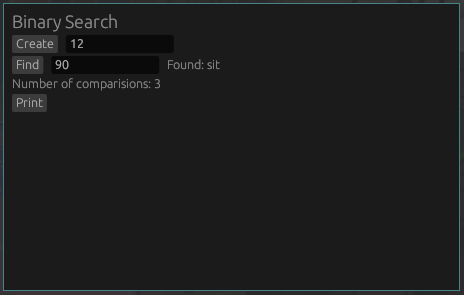
\includegraphics[scale=0.7]{1}
			\caption{Вигляд програми}
		\end{figure}
		
		\begin{figure}[H]
			\centering
			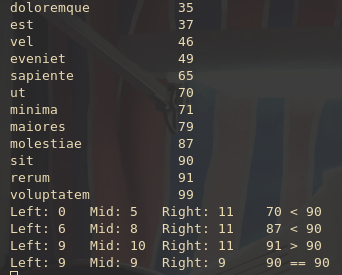
\includegraphics[scale=0.7]{2}
			\caption{Покроковий вивід}
		\end{figure}
	
	\begin{figure}[H]
		\centering
		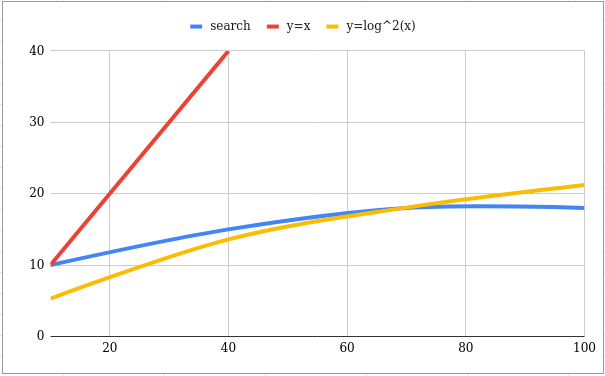
\includegraphics[scale=0.7]{3}
		\caption{Діаграма}
	\end{figure}
		
		\section*{Висновоки}
		Під час виконання лабораторної роботи я навчився застосовувати алгоритм бінарного пошуку при розв’язуванні задач та перевірити його ефективність на різних масивах даних. Експериментально визначив складність алгоритму. 
		
	\end{normalsize}
\end{document}
